\documentclass[conference]{IEEEtran}
\usepackage{graphicx}
\usepackage{tikz}
 
\usepackage[colorlinks = true, citecolor = blue]{hyperref}

% math lib
\usepackage{amsmath}
\usepackage{mathrsfs}

% operators
\DeclareMathOperator*{\argmax}{arg\,max}
\DeclareMathOperator*{\argmin}{arg\,min}
\newcommand\ceiling[1]{\left\lceil #1 \right\rceil}

% empty set
\usepackage{amssymb}
\let\emptyset=\varnothing

% algorithms
\usepackage{algorithm}
\usepackage{algorithmic}
\renewcommand{\algorithmicrequire}{\textbf{Input:}}
\renewcommand{\algorithmicensure}{\textbf{Output:}}

\begin{document}
% --------------------------------------------
% --------------Change HERE! -----------------
% --------------------------------------------
\def\authorone{Tom Odem}
\def\authortwo{Zixiao Fan}
\def\groupid{1}
% --------------------------------------------
\title{CS258 Final Report: The RSA Problem}
\author{
    \IEEEauthorblockN{\authorone\ and \authortwo}
    \IEEEauthorblockA{
        Group \groupid
    }    
}

\maketitle
\IEEEpeerreviewmaketitle


\section{Methods: RL-based Routing}
\subsection{RL Algorithms}
\begin{flushleft}
We chose two different RL algorithms to test our custom environments: Proximal Policy Optimization (PPO) and Monotonic Advantage Re-Weighted Imitation Learning (MARWIL). We chose PPO due to it already being implemented in the given code and its promising performance when testing our network environments. We chose MARWIL due to its hybrid imitation learning technique employed on historical data.
\end{flushleft}
% List RL algorithms and give a brief explanation of each




\subsection{State Space}
% Explain state/action/reward
% Make sure you provide enough information to reconstruct results
% Check https://gymnasium.farama.org/environments/box2d/lunar_lander/ for some examples
\begin{flushleft}
Our state space is made to represent the current options given to the agent in response to the current request. We initialize our environment with a list of every possible simple path that can be taken from any node to another. Each path is tracked as either "available" or "unavailable". When every color route on a path is unable to accommodate traffic, the path is deemed as unavailable. Path availability is updated whenever a request enters or leaves the network.
\end{flushleft}

\begin{flushleft}
When a new request is created, we identify which paths from the source to destination are available. Additionally, we sort the available paths into two categories: short or long paths. A short path is a path that takes 2 or less hops to complete, where a long path takes more than 2 hops. We chose 2 hops because on average 3 hops can connect most nodes, but 2 hops would limit the reachability of short paths. So, our state space reflects the state of what paths are available to the agent to travel from the request's source to destination.
\end{flushleft}

\begin{flushleft}
The state space is comprised of three discrete variables, each being set to either 1 or 0. The first variable is long\_available, which tells the agent that there is one or more long paths available to take to get from the source to destination. The second variable, short\_available, notifies the agent that there is one or more short paths that it can take to get from source to destination. The final variable is no\_path\_available, which explicitly tells the agent that there are no paths currently open to get from the source to destination.
\end{flushleft}

\begin{flushleft}
We chose to use this method because path availability can readily be computed with the propagated state information that our network simulation from the assignment assumes. Because this information can be readily computed, we can simply supply the agent with the state of whether or not any paths are available between the request's source and destination pair. This also allows the agent the freedom to take any path from source to destination without learning all 878 simple paths present within the network.
\end{flushleft}


\subsection{Action Space}
\begin{flushleft}
The action space is a discrete variable that can be 0, 1, or 2. A 0 signifies that the agent would like to take a short path. A 1 means the agent wants to take a long path. An action of 2 correlates to the agent choosing to block the current request. 
\end{flushleft}
\begin{flushleft}
Instead of simply giving the agent the possibility of choosing to take an available path or not, we introduce the option to take a short path or long path to allow the agent to optimize distance traveled. 
\end{flushleft}
\subsection{Reward Function}
\begin{flushleft}
Since the goal is to map the request onto the network, choosing a short or long path when they are set to 1 will give a positive reward. Choosing a long path when one is available will return a reward of 2. Since we also want the agent to optimize the amount of hops taken, choosing a short path when one is available will return a reward of 3. 
\end{flushleft}
\begin{flushleft}
If the agent chooses to take a short or long path and there are no corresponding length paths, it will receive a reward of -2. This is the worst option; If there are no path choices then the agent should choose to block instead of choosing an invalid path. Additionally, if there is only one length path available then it should choose that length path, not another one.
\end{flushleft}
\begin{flushleft}
When the agent blocks a request, it receives a reward of -1.
\end{flushleft}

\section{Method: Spectrum Allocation}
\begin{flushleft}
Since our agent is given a choice based on valid paths from source to destination, we can guarantee that the edges within a given valid path are free to use. Additionally, our model can take many different routes to get from source to destination. This gives us an abundant amount of options to choose from within the network to fulfill a request, especially compared to the low amount of traffic that can be present in the network at any time. Most nodes have multiple ways to reach them, which lets us leverage those plentiful path options. 
\end{flushleft}
\begin{flushleft}
Since our agent is given a choice based on valid paths from source to destination, we can guarantee that the edges within a given valid path are free to use. Additionally, our model can take many different routes to get from source to destination. This gives us an abundant amount of options to choose from within the network to fulfill a request, especially compared to the low amount of traffic that can be present in the network at any time. Most nodes have multiple ways to reach them, which lets us leverage those plentiful path options. 
\end{flushleft}
\begin{flushleft}
Because of these observations, we found that we only needed a simple spectrum allocation function. Thus, we use the simple and trustworthy greedy allocation method to choose the first available color within a path's edges. If a path's edges have no available colors, we can simply take a different path that is available to route around the blockage. This is highly flexible, as it does not matter where a blockage occurs. A majority of the time there are many other paths to choose from, so we can simply route around the blockage with an available path.
\end{flushleft}


\section{Results}
\begin{flushleft}
To gather data, we saved the results of every training round within the algorithm.train() function. A training round in this context is all 100 episodes that the environment runs for, thus encapsulating all 100 requests per training round. To get the data, we write to a .csv file from within the environment when the environment terminates.
\newline \newline 
We trained the PPO algorithm for both random routes and the single route environments for 10 iterations. The PPO algorithm runs 40 training rounds per iteration, giving us a total of 400 training rounds and 40,000 episodes.
\newline \newline
We trained the MARWIL algorithm for both random routes and the single route environments for 10 iterations. The MARWIL algorithm runs 2 training rounds per iteration, giving us a total of 20 training rounds and 2,000 episodes.
\newline \newline
\textit{Note: Red lines in graphs signify the average of the y axis variable when the model converges. For PPO, convergence occurred at training episode 200. For MARWIL, convergence occurred at training episode 17}
\end{flushleft}
\subsection{Learning Curve}


% Insert figures
\begin{flushleft}

\underline{PPO Random Routes and Single Routes}
\begin{figure}[ht!]
    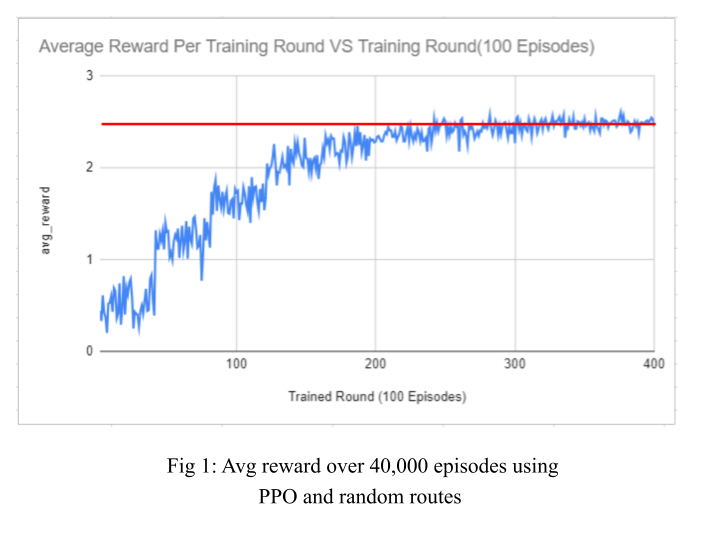
\includegraphics[width=.75\linewidth]{Final Paper Results And Graphs.png}
\end{figure}
\newline

Fig 1 shows the results from training using the PPO algorithm and random routes at each generate request. The model converges to an average average-reward of 2.44. This tells us that the model learned that taking short paths is a better choice when available. Thus, not only does our model adequately learn to route to other destinations, it also learns to prioritize paths with less hops.
\begin{figure}[ht!]
    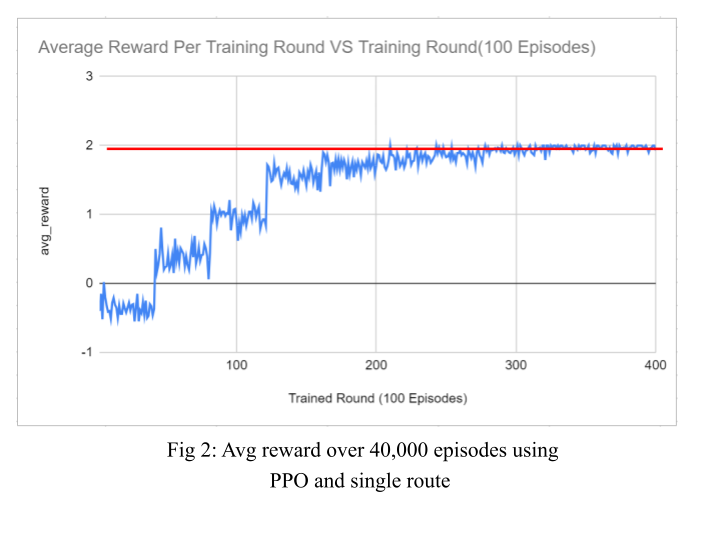
\includegraphics[width=.75\linewidth]{Final Paper Results And Graphs (2).png}
\end{figure}
\newline

Fig 2 shows the results from training using the PPO algorithm and a single route at each generate request. The model converges to an average average-reward of 1.96. Here we can see a large decrement compared to the previous average average-reward using random route. With a reward so close to 2, we can assume that it chose longer paths a majority of the time. This makes sense, as there are very few short paths on the specified single route, leading to the short paths being filled quickly and leaving the model with only long paths. So while the average-reward went down, it still performed optimally and found a path a majority of the time.
\end{flushleft}

\begin{flushleft}
\underline{MARWIL Random Routes and Single Routes}
\begin{figure}[ht!]
    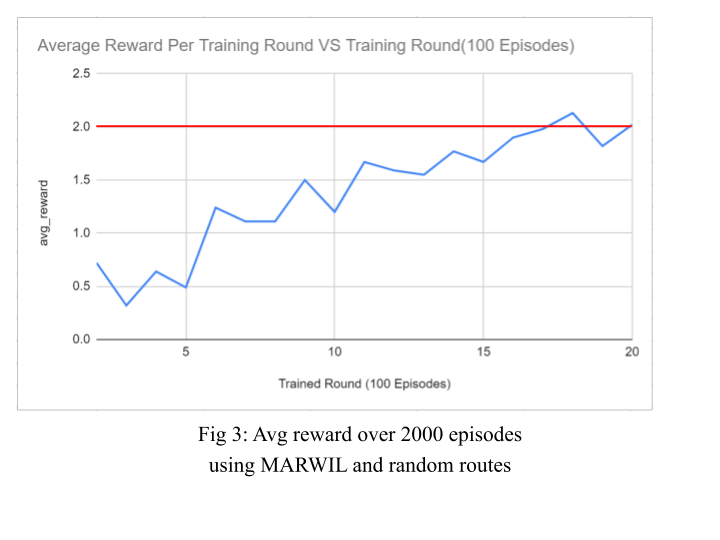
\includegraphics[width=.75\linewidth]{Final Paper Results And Graphs (4).png}
\end{figure}
\newline
Fig 3 shows the results from training using the MARWIL algorithm and random routes at each generate request. The model converges to an average average-reward of 2.02. When comparing to PPO's random route algorithm, there is a large difference. The MARWIL random route algorithm seems to have not learned to prioritize short paths over long ones, but due to the still relatively high average reward we can see that it is choosing an open path a majority of the time. The fact that the average reward is slightly over 2 means that the algorithm can choose a short path, albeit rarely.
\begin{figure}[ht!]
    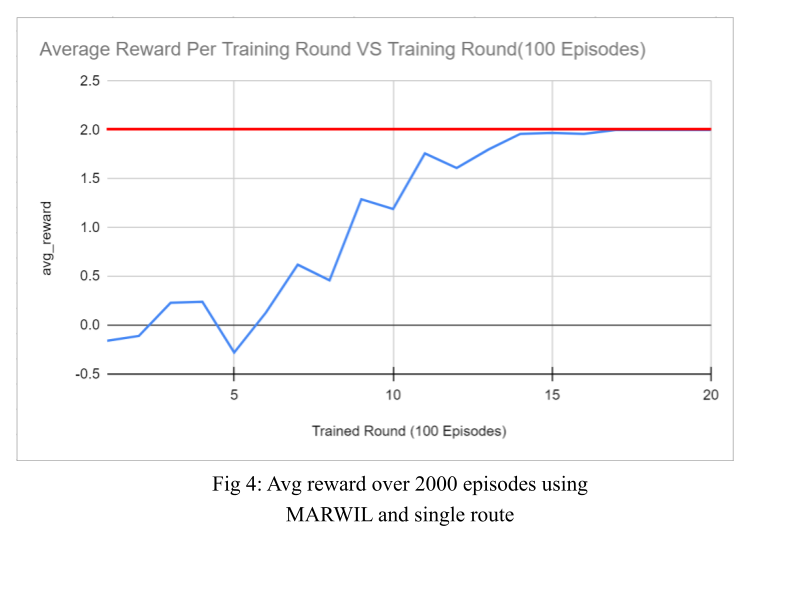
\includegraphics[width=.75\linewidth]{Final Paper Results And Graphs (6).png}
\end{figure}
\newline
Fig 4 shows the results from training using the MARWIL algorithm and a single route at each generate request. The model converges to an average average-reward of 1.99. While slightly worse than the previous MARWIL algorithm, it's performance shows the same trend; The algorithm learned to choose open paths and not to choose closed paths or block valid requests. Just like the PPO's single route algorithm, it primarily uses long paths due to the very limited short paths available to it.
\end{flushleft}




% Explain the results

\subsection{Utilization (The Objective)}
\begin{flushleft}
\underline{PPO Random Routes and Single Routes}
\begin{figure}[ht!]
    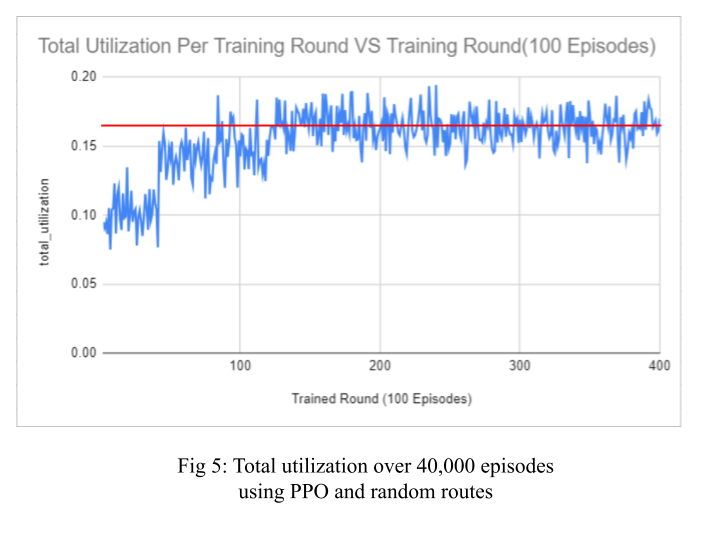
\includegraphics[width=.75\linewidth]{Final Paper Results And Graphs (1).png}
\end{figure}
\newline \newline
Fig 5 shows the results from training using the PPO algorithm and random routes at each generate request. The model converges to an average total utilization of .164. As we can see, the model converged very quickly to this utilization. Comparing this to Fig 1, we can see that the model quickly learned to choose open paths, but took a bit longer to learn to to prioritize short paths. 
\newline \newline
\newline \newline
\newline \newline


\begin{figure}[ht!]
    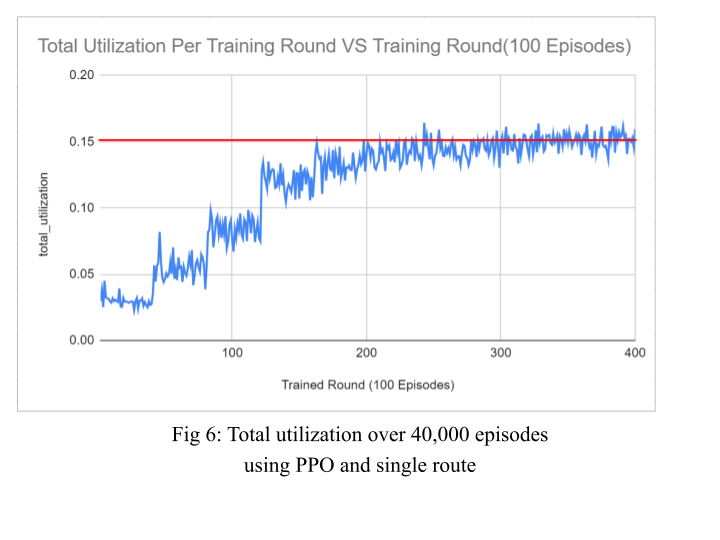
\includegraphics[width=.75\linewidth]{Final Paper Results And Graphs (3).png}
\end{figure}
Fig 6 shows the results from training using the PPO algorithm and a single route at each generate request. The model converges to an average total utilization of .15. This is not far off from the .164 from the PPO random route algorithm, and could be different due to the randomness of the holding time. However, from the graph we can see that it reached convergence much slower, which suggests that it was harder for the algorithm to learn to choose valid paths over invalid ones or blocking. This could mean that the algorithm simply hadn't learned as well as the PPO random route algorithm and could also explain the difference.

\end{flushleft}
\begin{flushleft}
\underline{MARWIL Random Routes and Single Routes}
\begin{figure}[ht!]
    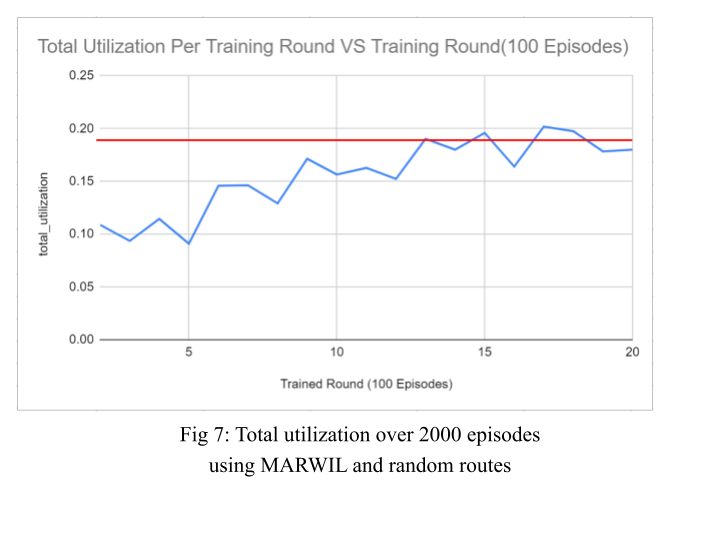
\includegraphics[width=.75\linewidth]{Final Paper Results And Graphs (5).png}
\end{figure}
\newline \newline
Fig 7 shows the results from training using the MARWIL algorithm and random nodes at each generate request. The model converges to an average total utilization of .187. This is better than the PPO random route algorithm's results, which could point to MARWIL more effectively learning to pick valid paths. Again, the randomness of holding times could cause this, but the difference is quite big. It is interesting to note that this model outperformed the PPO random route algorithm in total utilization, but was significantly worse when it came to average average-reward. This MARWIL algorithm may have learned to better utilize long paths to ensure utilization, rather than trying to use short paths to obtain less hops.
\newline \newline
\newline \newline
\newline \newline

\begin{figure}[ht!]
    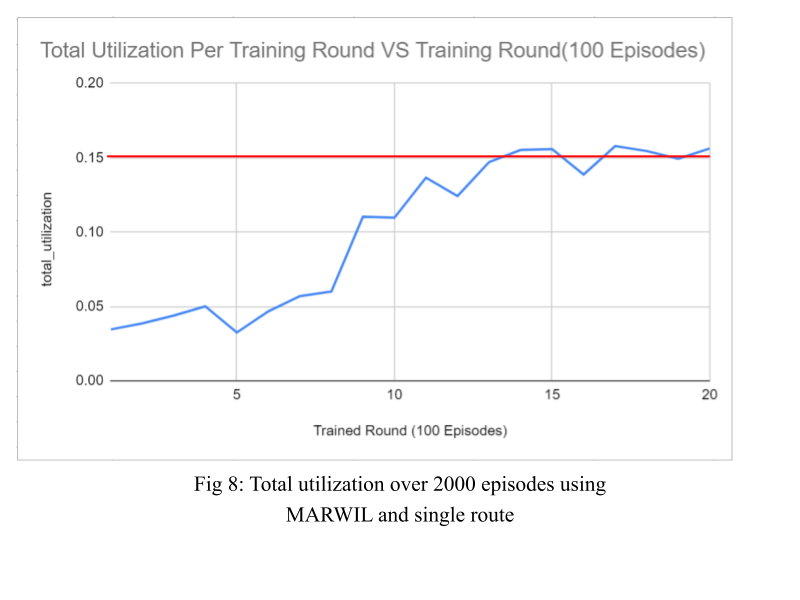
\includegraphics[width=.75\linewidth]{Final Paper Results And Graphs (7).png}
\end{figure}
Fig 8 shows the results from training using the MARWIL algorithm and a single route at each generate request. The model converges to an average total utilization of .15. This is the same utilization that the PPO single route achieved, so both are equally as good at selecting paths when dealing with single routes. This also means that both are worse at managing utilization than the random route alternatives, though the same reasons covered in the PPO single route algorithm could explain this discrepancy as well. This algorithm is also slower to converge, further enforcing the idea that the single route algorithms don't learn as well as their random route counterparts. 
\end{flushleft}
\subsection{Comparison}
We refer to the simple shortest path + index-based allocation strategy as a baseline case. The average total utilization is around 0.0615 for the random source/destination case(case 2) and 0.060 for the specified source/destination case(case 1).

Comparing our methods to the baseline, MARWIL earned a total utilization score of .187 for case 2, achieving over a 300\%  performance improvement. For case 1, MARWIL acquired a total utilization score of .15,  giving a 250\% boost in performance. PPO gave a total utilization of .164 for case 2, accomplishing an over 250\% improvement.Finally, PPO obtained a total utilization score of .15 in case 1, giving us a 250\% improvement. Overall, our methods ranged from achieving a 250\% to an over 300\% improvement over the shortest path + index-based allocation strategy.


\end{document}



